\documentclass{article}
\usepackage[sorting=none]{biblatex}
\usepackage{graphicx} % Graphics: https://www.overleaf.com/learn/latex/Inserting_Images
\usepackage{titlesec} % Subsections
\usepackage{mathtools} % https://tex.stackexchange.com/questions/268766/curly-braces-in-math-mode
\usepackage{hyperref} % https://tex.stackexchange.com/questions/73862/how-can-i-make-a-clickable-table-of-contents
\usepackage{amsmath}
\usepackage{amsfonts}
\usepackage{xcolor}
\usepackage{xparse}
\usepackage{algorithm}
\usepackage{algpseudocode}

\addbibresource{sources.bib}
\graphicspath{{figures/}}
\makeatletter % https://tex.stackexchange.com/questions/2651/should-i-use-center-or-centering-for-figures-and-tables
\g@addto@macro\@floatboxreset\centering
\makeatother
\DeclarePairedDelimiter\set\{\}
\hypersetup{
    colorlinks,
    citecolor=black,
    filecolor=black,
    linkcolor=black,
    urlcolor=black
}

% Use with dfrac
% https://tex.stackexchange.com/questions/33502/vertical-spacing-between-fractions-in-matrix-environment
\renewcommand{\arraystretch}{2.5}

\NewDocumentCommand{\codeword}{v}{%
\texttt{\textcolor{blue}{#1}}%
}

% Color a variable
\newcommand{\colorvar}[2]{
	\begingroup\color{#1}{#2}\endgroup
}

% Titular information
% https://en.wikibooks.org/wiki/LaTeX/Title_Creation
\title{
	An Undergraduate's Explanation of the Multilayer Perceptron: 
	Mathematical Concepts and a Python3 Implementation}
\date{2022 \\ January}
\author{Jared Frazier\thanks{Department of Computer Science (2021-2022),
Middle Tennessee State University.} \thanks{Department of Chemistry (2018-2021),
Middle Tennessee State University.} \thanks{Not endorsed by or affiliated with any of the 
authors or entities listed in the References section.}}

% Document 
\begin{document}
\maketitle
\titlepage

% https://www.overleaf.com/learn/latex/Table_of_contents
\tableofcontents
\pagebreak

\section{Preamble}
\quad The purpose of the present document is to explain and implement the major mathematical
constructs/concepts behind feedforward neural networks, specifically the multilayer perceptron.
This includes the layers that compose such networks, the cost (aka loss, error, or objective) function
and activation functions, the forward pass through the network,
the computation of gradients via backpropagation (a concept that is often "handwaved" to the extreme
or explained in so much detail as to be utterly confusing--at least in my experience),
and the update of model parameters via mini-batch stochastic gradient descent.
If the ideas such as \textit{layer} and \textit{backpropagation} are entirely unfamiliar
to you, then I encourage you to visit 3Blue1Brown's Deep Learning YouTube Series \cite{3Blue1BrownWhatIsANN2017}
and peruse the first few chapters of texts such as \textit{Deep Learning} (free, online) \cite{Goodfellow2016},
\textit{Neural Networks and Deep Learning} (free, online) \cite{Nielsen2015},
\textit{Hands-on Machine Learning with Scikit-Learn, TensorFlow and Keras 2ed} (buy) \cite{Geron2020},
and/or \textit{Deep Learning with Python 2ed} (buy) \cite{Chollet2021}. The present document
is not intended to be a comprehensive overview of neural networks nor an extremely
in-depth mathematical treatise but rather a document that highlights certain concepts that
I found confusing or ambiguous when I was first learning about neural networks,
particularly regarding the backpropagation algorithm.

Having taken my institution's CSCI 4350 (Intro to AI) and CSCI 4850 (Neural Nets)
courses in addition to conducting independent research using
variational autoencoders, recurrent neural nets, convolutional neural nets, and
self-attention, I am ashamed to say my fundamental understanding of neural nets
was far weaker than it should have been. While I am not a master of pedagogy,
I hope this document will serve as a reminder of fundamental concepts for my
future self and for others.

\section{Introduction}

\quad The neural network (function approximator) is just a chain of geometric transformations (functions)
each parametrized by a weight matrix $W \in \mathbb{R}^{n_h \times n_x}$ and
a bias vector $b \in \mathbb{R}^{n_h}$ on the input vector $x \in \mathbb{R}^{n_x}$.
The geometric transformations of the neural network are encapsulated by connecting
layers (e.g., dense/fully connected layers) together. A neural network has $L$ total
layers and the current layer $l$ receives the output from the previous layer $(l-1)$.
Note that $n_x$ is the number of features (or independent variables) in the input
and $n_h$ is the number of hidden units in the current layer. The following subsections will
briefly elucidate both the claims and notation of the first sentence of this section.

\subsection{Parametrized Functions}

\quad I assume you know what a function is; however, the term \textit{parametrized}
is one that appears often in deep learning literature and should be well-understood by the student.
Consider a generic quadratic function \cite{MathSEVarsParamsArgs2015} as
% Quadratic function
\begin{equation}
	f(x) = ax^{2} + bx + c
\end{equation}
The \textit{variable} $x$ is an \textit{argument} to the function $f$ that has
\textit{parameters} $a$, $b$, and $c$. The parameters determine the behavior of
the function (e.g., the steepness of slope, intercepts, shape, etc.) while the
variable can take on some range of values. When a variable that takes on a particular
value is passed as an argument to the function with defined parameters, the result
is some other value $y$ if $y = f(x)$. This explanation of a function
should not be anything new; however, the \textit{parameters} are quantities
of particular interest for neural networks since the parameters are the quantities
that are \textit{learned} by the neural network over time. What it means to learn
parameters will be explained later.

A neural network can be denoted as a function $h$ with parameters $W$
and $b$ of a variable $x$. This statement can be compactly written as
$h_{W, b}(x)$ as in \cite{Geron2020} or $h(x; W, b)$ as in \cite{Goodfellow2016}.
Incidentally, I encourage you to know both notation, but the former appears to be more common
in general in addition to being quite common for specialized
probabilistic models such as the variational autoencoder \cite{Kingma2014}.
The subscript with $W$ and $b$ means that the weights $W$ and biases $b$ are
\textit{parameters } of the neural network $h$.
The claim that a neural network is a chain of functions is useful later during
the updating of the parameters of the network. To briefly illustrate the idea
of chaining functions, the generic quadratic function, which can be defined
as a composite function $f$, can be decomposed into simpler functions shown
below.

\begin{align}
	g_{a}(x)     & = ax^{2}                  \\
	u_{b}(x)     & = bx                      \\
	f_{a,b,c}(x) & = g_{a}(x) + u_{b}(x) + c
\end{align}
Recognizing the decomposition of composite functions into their constituent
functions is useful for applying rules of calculus--the basis of parameter learning via
the backpropagation algorithm illustrated later.

\subsection{Operand Types}

\quad The input $x$ is not a single value as is conceived in the elementary
formulations described above. Rather, the input $x$ is a list of
values referred to as a \textit{column vector}. Each element of the vector
is a value that a particular feature, or independent variable, could take on.
The shape of the vector $x$ is important to understand since the functions and operations
performed by the neural network (dot product, Hadamard product, addition, etc.)
restrict their vector/matrix operands to particular shapes. When using the term
\textit{vector}, I am always referring to a \textit{column vector}
unless otherwise specified. Also, note that $x \in \mathbb{R}^{n_x}$ indicates
that $x$ is a vector with $n_x$ elements and the $j^{th}$ element is a real number.
For example, the below vector $x$ is shown and a common vector operation
known as the transpose (converts a \textit{column vector} to a
\textit{row vector} and is denoted with a superscript $\top$) is also shown.
\begin{align}
	x & = \begin{bmatrix}
		x_{1}  \\
		x_{2}  \\
		x_{3}  \\
		\vdots \\
		x_{(n_x)}
	\end{bmatrix}
	=
	\begin{bmatrix}
		x_{0}  \\
		x_{1}  \\
		x_{2}  \\
		\vdots \\
		x_{(n_{x}-1)}
	\end{bmatrix}
	=
	\begin{bmatrix}
		x_{0} & x_{1} & x_{2} & \cdots & x_{(n_{x}-1)}
	\end{bmatrix}^\top
\end{align}

Many programming languages access the first element of a vector using the index
0; this notation is shown above in addition to the more standard
mathematical notation where the first element begins with the index 1.
For the remainder of this document, I will use the index 0 assumption
since my implementation of the neural network uses the Python
programming language. If you wish to implement the same algorithms in a language
such as R or Wolfram Mathematica, be wary of this index discrepancy.
Consequently, with the index beginning at 0, the last index of a vector with
$n_x$ elements will be $(n_x - 1)$... and woe is the programmer who commits an
off-by-one error.

A matrix $W$ represents the weight of edges between the $k^{th}$
input neuron of $n_x^{l-1}$ total input neurons (i.e., neurons in the previous layer $(l-1)$)
and the $j^{th}$ hidden neuron of $n_h^{l}$ total hidden neurons in the current layer $l$.
A weight matrix looks similar to the vector, except rather than having a single
column, a matrix has a rows and columns--looking like a table. Vectors can
be referred to as rank-1 tensors, matrices as rank-2 tensors, so-on and so-forth
for multiple index "lists" in higher dimensions. A sample weight matrix
$W \in \mathbb{R}^{n_h \times n_x}$ is shown below.

\begin{align}
	W & = \begin{bmatrix}
		W_{00}         & W_{01}         & W_{02}         & \cdots & W_{0(n_{x}-1)}         \\
		\vdots         & \vdots         & \vdots         & \vdots & \vdots                 \\
		W_{(n_{h}-1)0} & W_{(n_{h}-1)1} & W_{(n_{h}-1)2} & \cdots & W_{(n_{h}-1)(n_{x}-1)}
	\end{bmatrix}
\end{align}

When implementing machine learning algorithms, pay close attention to the
input and output shapes described in a dataset, journal article, tutorial, or
the source code of others. If you do not pay careful attention to these shapes,
your implementation may not run or, worse, it \textit{will} run but it will not execute
the operations you intended\footnote{This is especially true for the
	matrix multiplication operation and the Hadamard (element-wise) product.}.

\section{The Multilayer Perceptron}

\quad Here I define the operations that occur for the multilayer perceptron (MLP).
Note that the MLP can sometimes refer to any class of feedforward
neural network, that is a network that applies affine transformations and
activation functions to input from a previous layer in the network.

\subsection{The Dense/Fully Connected Layer}

\quad The affine transformation, which is the most fundamental transformation
of the densely/fully connected layers that exist in the MLP, yields
a weighted input vector $z^{l}$ with elements
$z_j^{l} = W_{jk}^{l} a_{k}^{l-1} + b_{j}^{l}$ for a layer $l$ and neuron $j$.
Here, the activation $a_k^{l-1}$ denotes the activation of the $k^{th}$ neuron of the
previous layer $(l-1)$. Importantly, the input layer has no activation function $\phi$
associated with it, so the activation vector $a^{0}$ equals the input vector $x$.
Moreover, the inner dimensions of the matrix product
$Wx$ match, that is the subscripts $k$ are "adjacent" to one another. While you may
observe that the activation vector $a^{l} \in \mathbb{R}^{n_a}$ is clearly not a matrix,
numerical libraries will often treat a vector $v \in \mathbb{R}^{n_v}$ as equivalent
to a matrix with a single column (i.e., $V \in \mathbb{R}^{n_v \times 1}$) for
the purposes of performing fast matrix-matrix calculations.

Until now the discussion of the MLP has been entirely in abstract mathematical
notation, so now a visual of a single layer (meaning single hidden layer)
MLP is shown. The activation function $\phi$ is vectorized, meaning it
applies to each element of a vector, matrix, or rank-n tensor. Vectorized
activation functions are often denoted $\phi(\cdot)$ or $\sigma(\cdot)$, though I do not like
the latter notation as $\sigma$ typically references the sigmoid function. The number of
neurons in a hidden layer (or output layer for that matter) $n_h$ does not have
to be constant, and this is shown in the Figure 1 below where the output layer
has only a single neuron while the hidden layer has three neurons.

% Multilayer perceptron figure
\begin{figure}[h]
	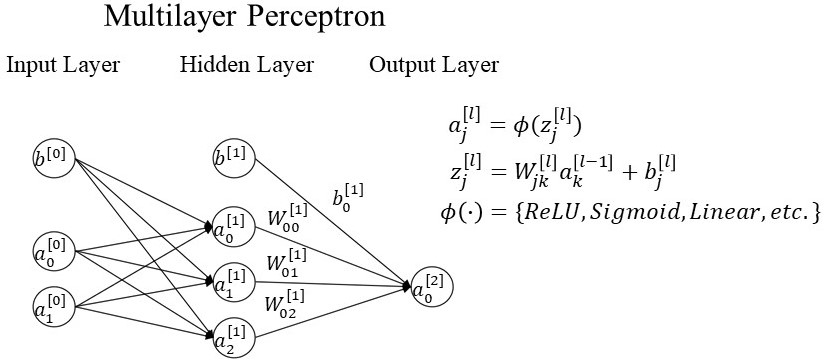
\includegraphics[scale=0.60]{mlp_larger_font_croppped.jpg}
	\caption{The multilayer perceptron with bias vectors $b$ in layers
		$[l]$ and activations $a$ for the $j^{th}$ neuron in a layer. The weights
		$W$ of the last layer are shown as edges connecting neurons in the hidden
		layer to the output layer. The operations are defined to the right
		of the figure along with a set of
		common vectorized activation functions $\phi(\cdot)$.}
\end{figure}

% Multilayer percetpron with useneuralnetwork pkg
% \begin{align}
% 	\begin{neuralnetwork}[height=3, layertitleheight=5.0em]
% 		\newcommand{\x}[2]{$a^{0}_#2$}
% 		\newcommand{\hfirst}[2]{\small $a^{(1)}_#2$}
% 		\newcommand{\y}[2]{$a^{2}_#2$}
% 		\inputlayer[count=2, bias=false, title=Input Layer 0, text=\x, nodeclass={input neuron}]
% 		\hiddenlayer[count=3, bias=false, title=Hidden Layer 1, text=\hfirst, nodeclass={hidden neuron}] \linklayers
% 		\outputlayer[count=1, title=Output Layer 2, text=\y, nodeclass={output neuron}] \linklayers
% 	\end{neuralnetwork}
% \end{align}

\subsection{The Forward Pass and Cost Function}

\quad The MLP is a function approximator and the MLP learns the parameters of
this function. Since the learning is just the determination of the values of the
parameters of the MLP, then there must be some other function that determines
how well the parameters of the MLP approximate the desired function. This other
function is called the cost or loss function and is denoted $C$, though sometimes
it is denoted $\mathcal{L}$ or $J$\footnote{Despite these functions sharing the same notation as
	a matrix $W$, the result of the function is not a tensor but is rather a scalar.}.
For regression problems, the most common
cost function is the mean squared error. The cost function, unlike previous
operations, returns a scalar and \textit{not} a vector. The scalar value can be used to estimate
performance during training; however, when implementing backpropagation, you will
be more interested in the derivative of the cost with respect to certain variables
and using gradient vectors (discussed later) rather than the scalar cost.

\begin{equation}
	\begin{aligned}
		C & = \frac{1}{N} \sum_{x} {C_x}                       \\
		  & = \frac{1}{N} \sum_{x} {||(\hat{y} - y)||^{2} }    \\
		  & = \frac{1}{N} \sum_{x} {||(h_{W,b}(x) - y)||^{2} } \\
		  & = \frac{1}{N} \sum_{x} {||(a^{L} - y)||^{2} }
	\end{aligned}
\end{equation}

where $x$ and $y$ are in $\mathbb{R}^{n_x}$ and

\begin{equation}
	||x - y||^{n} = \sum_{i=0}^{n_{x}-1} { (x_{i} - y_{i})^{2} }
\end{equation}

The cost function for a single sample $C_x$ is a multivariable function
and it can also be written as a function of its parameters $\theta$ like
$C_x(\theta)$ where $\forall$ layers $l,\ \theta = \set{W^{l}, b^{l}}$. Additionally,
$C_x$ can be written to emphasize a certain parameter such as the weight $C_x(W)$.
More importantly, the derivative of the cost function $C_x$ with respect the activation
$a_j^{L}$ for the $j^{th}$ neuron of the last layer (i.e., output layer) $L$ is defined as
$\frac{\partial C_x}{\partial a_j^{L}}$. To avoid long superscripts, assume
that the the last layer $L$ actually indexes the location $(L-1)$.
These partial derivatives are relevant to the backpropagation algorithm illustrated shortly.

Before moving on to backpropagation, I briefly explain the meaning of the activations
of the last layer. Put simply, The activation vector $a^{L}$ for the last layer $L$ is the prediction
that the MLP makes. The activation vector $a^{L}$ has a number of elements
determined by the number of units $n_h^{L}$ in the last layer, and to index the $j^{th}$
activation (a scalar) of the activation vector one would write $a_j^{L}$. The activation for
the $j^{th}$ neuron is used to compute errors that are relevant for the
backpropagation algorithm since how well $a^{L}$ "lines up" with the known
result $y$ is determined by the choice of parameters $W$ and $b$ for all layers $l$.
Here I loosely use the phrase "lines up" because $a^{L} = \hat{y}$ and for supervised
learning problems, it is desirable for $\hat{y}$ to be very "close" to $y$. Of
course, the metric for such "closeness" is the cost function!

\subsection{Backpropagation}

\quad The key to learning for the MLP, and for artificial neural networks in general,
is updating the weights $W^{l}$ and biases $b^{l}$ for each layer $l$ such
that the network performs better with respect to the loss function\footnote{
Machine learning APIs like TensorFlow tend to formulate cost functions
such that they can be \textit{minimized} (e.g.,
$minimize(NegativeLogLikelihood) \equiv maximize(LogLikelihood)$)}.
Since $W$ and $b$ are tensors, the gradients\footnote{Denoted
	using the gradients $\nabla$ or sometimes the $\vec{\nabla}$ operator.}
of the cost function with respect to these parameters ($\frac{\partial C_x}{\partial W_{jk}^{l}}$
and $\frac{\partial C_x}{\partial b_{j}^{l}}$) are computed to determine how
the elements of the parameter tensors should be modified to produce better predictions.

\subsubsection{Parameters Revisited}

\quad At this point you might ask yourself again what the difference between
variables and parameters is. In pure mathematics classes, you are often asked
to minimize a function with respect to some variable(s), and rarely (at least in
my experience) with respect to a parameter. Why minimize the cost
function with respect to the parameters? The statement "minimize with respect
to a parameter" seems to contradict the very definition of a parameter:
"arguments that are... not explicitly varied in situations of interest are termed
\textit{parameters}" \cite{WolframMathWorldParameterDefinition}. The simplest intuition
behind the minimization of parameters instead of variables
is that the parameters are constant for a single iteration
of a machine learning experiment, and then updated such that the model performs
better on future experiments. Conversely, variables (e.g., the input $x$) are
independent of the model. An experiment encompasses the \textit{fitting} of a
model for a number of iterations equal to
$NumEpochs \times \frac{TrainingDataSize}{BatchSize}$. A \textit{batch} for learning
is just a random subset of size $m$ of the training data. Thus, one iteration of the
machine learning experiment is performing the forward pass (i.e., making a prediction
$a^{i, L} = y^{i}$ for each training example $x^{i}$ in the batch),
computing the gradients for the weight matrices and biases of each layer based on the
model error, and then updating those parameters.

\subsubsection{Typical Mathematical Notation for Gradient Descent}

\quad Knowing that the parameters need to be updated, most often the below equations
will be written and the gradient computation process will be abstracted from
the reader.

\begin{align}
	W^{l}      & = W^{l} - \eta \nabla_{W^{l}}C           \\
	b^{l}      & = b^{l} - \eta \nabla_{b^{l}}C           \\
	\theta^{l} & = \theta^{l} - \eta \nabla_{\theta^{l}}C
\end{align}
The equations make quite a lot of sense if you think about exactly
what they are saying. The first of the three equations says "update the
weight matrix for a given layer by subtracting from the current weight matrix
the gradient of the cost function with respect to that same weight matrix." By definition,
the gradient points in the direction of local maxima, and the
negative gradient points in the direction of local minima \cite{MathLibreGradient2021}.
The size of the "step" in the direction of the local minima
is proportional to the learning rate $\eta$,
which is a hyperparameter (a parameter explicitly set by a user) of the model.
Therefore, the semantic explanation of the equations is essentially to change the
weights and biases (sometimes combined and denoted as a single parameter tensor $\theta$)
of the model by a small amount until convergence\footnote{Ideally
	on a global minimum in the N-dimensional cost function space.} is reached. In this way, a model
will have parameters that can be used to \textit{infer} predictions based on
unseen data. Consequently, when a model is making predictions without
updating the parameters, it is called \textit{machine learning inference} or
some variation on the word \textit{inference}.

\subsubsection{The Four Fundamental Equations of Backpropagation}

\quad While the previous equations are nice for rapidly intuiting the meaning of
gradient descent, they provide no insight into the computation of \textit{gradients}
that are obviously needed for \textit{gradient} descent.

The fundamental equations of backpropagation, which are critical for \textit{gradient}
descent, are claimed without proof (see \cite{Nielsen2015} for proofs). While
the previous equations are the "pretty" form of gradient descent, for the
accompanying implementation, one does not compute the gradient vectors of these parameters
directly, rather the components of these gradient vectors $\nabla_{W}C$ or $\nabla_{b}C$
are computed using other outputs of the network such as $a^{l}$ and $z^{l}$.


\begin{align}
	\delta^{L}                            & = \nabla_{a^{L}} \text{C} \circ \frac{\partial \phi}{\partial z}(z^{L})                                                                                                         \\
	\delta^{l}                            & = ((W^{l+1})^{\top} \delta^{l+1}) \circ \frac{\partial \phi}{\partial z}(z^{l})                                                                                                 \\
	\frac{\partial C}{\partial b_j^{l}}   & = \delta_j^{l}                                                                                                                                                                  \\
	\frac{ \partial C }{ \partial W^{l} } & = \delta^{l} (a^{l-1})^{\top}                                                   & \text{$\delta^{l} \in \mathbb{R}^{j \times 1}; (a^{l-1})^{\top} \in \mathbb{R}^{1 \times k}$}
\end{align}

Before explaining the meaning of the above equations,
consider first the gradient for a function $f$ of two variables $x$ and $y$:

\begin{align}
	f(x, y)        & = x^{2} y                                                                      \\
	\nabla f(x, y) & = \langle \frac{\partial f}{\partial x}, \frac{\partial f}{\partial y} \rangle \\
	\nabla f(x, y) & = \langle 2xy, x^{2} \rangle
\end{align}
You can see that the gradient is the vector where each element is the first-order
partial derivative with respect to each variable in the function $f$.

Now, consider the error vector $\delta^{L}$ for the last layer $L$ and note the gradient operator
$\nabla_{a^{L}}$ is with respect to the activation vector $a^{L}$ whose elements
can be defined as $a^{L} = \set{a_j^{L}}_{j=0}^{n_h - 1}$.
Thus, the error vector for the last layer is shown below for clarity. Assume that the cost
function $C$ is for a single example $x$ and $\delta^{L} \in \mathbb{R}^{n_y}$
where $n_y$ is the number of targets (or output classes).

\begin{align}
	\delta^{L} & =
	\begin{bmatrix}
		\delta_0^{L} \\
		\delta_1^{L} \\
		\delta_2^{L} \\
		\vdots       \\
		\delta_{(n_{y} - 1)}^{L}
	\end{bmatrix}
	=
	\begin{bmatrix}
		\dfrac{\partial C}{\partial a_{0}^{L}}(a_{0}^{L}) \dfrac{\partial \phi}{\partial z}(z_{0}^{L}) \\
		\dfrac{\partial C}{\partial a_{1}^{L}}(a_{1}^{L}) \dfrac{\partial \phi}{\partial z}(z_{1}^{L}) \\
		\dfrac{\partial C}{\partial a_{2}^{L}}(a_{2}^{L}) \dfrac{\partial \phi}{\partial z}(z_{2}^{L}) \\
		\vdots                                                                                         \\
		\dfrac{\partial C}{\partial a_{(n_{y} - 1)}^{L}}(a_{(n_{y} - 1)}^{L}) \dfrac{\partial \phi}{\partial z}(z_{(n_{y} - 1)}^{L})
	\end{bmatrix}
\end{align}

Showing the elements of the error vector $\delta^{L}$ above demonstrates what must be computed:
${\frac{\partial C}{\partial a_{j}^{L}}\ \text{and}\ \frac{\partial \phi}{\partial z}}$.
The derivative of the activation function $\frac{\partial \phi}{\partial z}$ is
very easy to compute since activation functions with well-known derivatives are
typically selected. For example, if the activation function is the sigmoid function,
then the derivative is known and shown below.

\begin{align}
	\phi(z)                             & = \frac{1}{1 + e^{-z}}      \\
	\frac{\partial \phi}{\partial z}(z) & = \sigma(z) (1 - \sigma(z))
\end{align}

The derivative of the cost function with respect to activations of different
neurons ${\frac{\partial C}{\partial a_{j}^{L}}}$ is also easily computed.
For the mean squared error function, you would derive the function with respect
to only a single activation. That is,
you are finding the rate of change of the cost function for an infinitesimally
small change in the $j^{th}$ activation of a layer.

\begin{align}
	C                                     & = \frac{1}{n_h} \sum_{j=0}^{(n_h - 1)} { (a_{j}^{L} - y_j)^{2} }                \\
	\frac{\partial C}{\partial a^{L}}     & = \frac{1}{n_h} \sum_{j=0}^{(n_h - 1)} { \frac{\partial C}{\partial a_{j}^{L}}} \\
	\frac{\partial C}{\partial a_{j}^{L}} & = 2(a_{j}^{L} - y_j)
\end{align}

You might ask yourself, "how do I actually get
$\frac{\partial C}{\partial a_{j}^{L}}$." Initially, I assumed the answer would
be something quite confusing, but when computing such a derivative, you need
only consider what a function is. If you think of $\frac{\partial C}{\partial a_{j}^{L}}$
as just another function, which it is, then of what variables is it a function?
It is simple: $a_{j}^{L}$ and $y_j$! We \textit{know} the values of these variables
since we know $a_{j}^{L}$ is just the output of a single neuron in a layer
of neurons. Moreover, $y_j$ is not something we have to compute, but rather it
is a known element of a vector of targets $y$, or desired outcomes.

Now, why does $\nabla_{a^{L}} C$ specify $a^{L}$? It is because $C$ can be written as
a function of many parameters and variables, and you only care about certain variables
when performing backpropagation. A single layer neural network,
that is a network with two weight matrices $W^{0}$ and $W^{1}$; two bias vectors
$b^{0}$ and $b^{1}$; and three activations $a^{0}$, $a^{1}$, and $a^{2}$
can be written as $C(W^{0}, W^{1}, b^{0}, b^{1}, a^{0}, a^{1}, a^{2})$. You might
note that the number of activation vectors $a$ exceeds the number of weight matrices
and bias vectors. Recall that the input layer of the MLP has no preceding
weight matrix, and a linear activation $\phi(x) = x$ is applied to the input vector,
thus resulting in activations $a^{0} = x$. Refer to Figure 1 to observe the lack
of a weight matrix before the input layer. The gradient must be taken with respect to a
certain parameter, otherwise the partial derivative with respect
to each variable of a vector valued function would result. To visualize what the gradient
only with respect to the activations of the last layer looks like, consider the below vector.

\begin{align}
	\nabla_{a^{L}} C & =
	\begin{bmatrix}
		\dfrac{\partial C}{\partial a_{0}^{L}} \\
		\dfrac{\partial C}{\partial a_{1}^{L}} \\
		\dfrac{\partial C}{\partial a_{2}^{L}} \\
		\vdots                                 \\
		\dfrac{\partial C}{\partial a_{(n_{h} - 1)}^{L}}
	\end{bmatrix}
\end{align}
The above vector is in stark contrast to $\nabla_{\theta^{L}} C$, where
$\theta^{L}$ are the relevant parameters and variables for the layer $L$.
Such a matrix is called the Jacobian matrix and is shown below.

\begin{align}
	\nabla_{\theta^{L}} C & =
	\begin{bmatrix}
		\dfrac{\partial C}{\partial a_{0}^{L}}           & \dfrac{\partial C}{\partial W_{00}^{L}}           & \dfrac{\partial C}{\partial W_{01}^{L}}         & \dfrac{\partial C}{\partial W_{0(n_{x}-1)}^{L}}         & \dfrac{\partial C}{\partial b_{0}^{L}}         \\
		\dfrac{\partial C}{\partial a_{1}^{L}}           & \dfrac{\partial C}{\partial W_{10}^{L}}           & \dfrac{\partial C}{\partial W_{11}^{L}}         & \cdots                                                  & \dfrac{\partial C}{\partial b_{1}^{L}}         \\
		\dfrac{\partial C}{\partial a_{2}^{L}}           & \dfrac{\partial C}{\partial W_{20}^{L}}           & \dfrac{\partial C}{\partial W_{21}^{L}}         & \cdots                                                  & \dfrac{\partial C}{\partial b_{2}^{L}}         \\
		\vdots                                           & \vdots                                            & \vdots                                          & \vdots                                                  & \vdots                                         \\
		\dfrac{\partial C}{\partial a_{(n_{h} - 1)}^{L}} & \dfrac{\partial C}{\partial W_{(n_{h} - 1)0}^{L}} & \dfrac{\partial C}{\partial W_{(n_{h}-1)1}^{L}} & \dfrac{\partial C}{\partial W_{(n_{h}-1)(n_{x}-1)}^{L}} & \dfrac{\partial C}{\partial b_{(n_{h})-1}^{L}}
	\end{bmatrix}
\end{align}

Now that you understand the computation of $\delta^{L}$, finding $\delta^{l}$
is trivial since the errors in the current layer plus one propagate backward through
the network (i.e., you will use $\delta^{L}$ in the computation of $\delta^{L-1}$).
To validate the shapes of the operands relevant to the equation for $\delta^{l}$,
refer to the below statements.

\begin{align}
	W^{l+1}                                 & \in \mathbb{R}^{\colorvar{red}{n_h^{l+1}} \times \colorvar{blue}{n_{h}^{l}}} \\
	\delta^{l+1}                            & \in \mathbb{R}^{\colorvar{red}{n_h^{l+1}}}                                   \\
	\frac{\partial \phi}{\partial z}(z^{l}) & \in \mathbb{R}^{\colorvar{blue}{n_{h}^{l}}}
\end{align}

With these comments about backpropagation,
the practical implementation of the four equations can be discussed.
Since the above equations focus on the computation of gradients,
they must be used in the \textit{gradient descent} equations below.

\begin{align}
	W^{l} & = W^{l} - \frac{\eta}{m} \sum_{x}{\delta^{x, l}(a^{x, l-1})^\top} \\
	b^{l} & = b^{l} - \frac{\eta}{m} \sum_{x}{\delta^{x, l}}
\end{align}

The learning rate $\eta$ is typically $\eta = \set{1^{i}}_{i=-2}^{-4}$, and $m$
for mini-batch stochastic gradient descent is typically
$m = \set{2^{i}}_{i=1}^{10}$.

\section{Implementation}

\quad Here I define the Python classes
that encapsulate the attributes (data members) and methods (functions) associated
with the MLP. Since this approach is object oriented, it was helpful to
define first the subunits of the MLP: operations (i.e., activation functions and
cost functions) and layers.

\subsection{Operation}

\quad The activation functions and cost functions are children of the Python
abstract base class I define as \codeword{Operation}. The
\codeword{Operation} has no arguments and initializes no attributes, but
does have a \codeword{__call__} method and \codeword{derivative} method. All
children of the \codeword{Operation} must implement these methods; however, if
the child is a \textit{cost function}, then this child class must also
implement a \codeword{gradient} method ($\nabla_{a^{l}}\text{C}$). The

\subsection{DenseLayer}

\quad The forward pass requires defining a class that
encapsulates the fully/densely connected layer of the MLP. I define this as
\codeword{DenseLayer} with attributes for the input dimensions $n_x$,
the weight matrix $W \in \mathbb{R}^{n_h \times n_x}$, and the bias
${b \in \mathbb{R}^{n_h}}$. The \codeword{DenseLayer} is correspondingly passed
arguments for $n_x$, $n_h$, and a \codeword{Callable}
that will be used as the vectorized activation function $\phi(\cdot)$ for a given layer.

The \codeword{__init__} method saves the \codeword{Callable} and passes
the $n_x$ and $n_h$ arguments to initialize the weight matrix and bias vector.
The \codeword{glorot_uniform} method initializes the values of the weight matrix
using Glorot Uniform initialization \cite{Glorot2010}. The bias vector is
initialized with zeros.

The activations and weighted inputs of the \codeword{DenseLayer}
are computed with the \codeword{__call__} method defined as

\begin{align}
	z & = XW^{\top} + b \\
	a & = \phi(z)
\end{align}
where $x$ is an argument to the \codeword{__call__} method and
$W$, $b$, and $\phi$ are attributes of the \codeword{DenseLayer}.
Note that $x$ can be $x \in \mathbb{R}^{n_x}$, which
is equivalent to ${X \in \mathbb{R}^{1 \times n_x}}$ for the purposes of matrix
multiplication. However, the training dataset $\mathcal{D}$ is commonly
$\mathcal{D} \in \mathbb{R}^{N \times n_x}$ where $N$ is the total number of
training examples. Therefore, a subset (aka batch) $m$ of $N$ means that
$X \in \mathbb{R}^{m \times n_x}$.

Consider now the shapes of the affine transformation and the subsequent activation:

% Determining shape of weighted matrix
\begin{align}
	Z_{m \times n_h} =
	X_{\colorvar{green}{m} \times \colorvar{red}{n_x}} (W_{\colorvar{blue}{n_h} \times \colorvar{red}{n_x}})^{\top} + b_{\colorvar{blue}{n_h}}
\end{align}
For this weighted input matrix $Z_{m \times n_h}$, you may observe a problem with how
it is computed:
a \textit{vector} is \textit{added} to a \textit{matrix}. This is an operation that is undefined.
While this operation is undefined, numerical libraries treat this as a legitimate
operation by \textit{broadcasting} the vector $b_{n_h}$ to $B_{m \times n_h}$ \cite{Goodfellow2016,NumPyBroadcasting2021}.

The activation matrix $A$ contains the activation vector as a row
for each training example and is expected to be $A \in \mathbb{R}^{m \times n_h}$
since it will be passed onto to the next layer as input.

\subsection{MLP}

The \codeword{MLP} encapsulates the \codeword{DenseLayer} objects and
implements a number of methods to approximate the function for a system.

The \codeword{__init__} method takes as arguments the dimension of the input
$n_x$, the number of units $n_h$ per hidden layer, the number of targets or
classes $n_y$, the learning rate $\eta$, the total number of hidden layers $l_h$,
the cost function $C$ as a string, activation function $\phi$ for hidden layers as a string,
and the activation function for the target layer $\varphi$ as a string. This method
also creates three \codeword{list} objects of particular important:
\codeword{sequential}, \codeword{activations_cache}, and
\codeword{weighted_inputs_cache} stored collectively as a \codeword{@property}
called \codeword{cache}. These \codeword{list} objects are used to
track the layers of the model, the activation vectors $a$ for a forward pass,
and the weighted input vectors $z$ for a forward pass.

The \codeword{fit} method takes inputs $X$, targets $y$, the batch size $m$,
and the number of epochs to train the model. Batching of the data occurs first.
This can be easily accomplished using \codeword{numpy.random.choice} with
the range of indices to sample from being the total number of training examples,
passing \codeword{replace=False}, and setting \codeword{size=(num_batches, batch_size)}.
The number of batches is $floor(\frac{\text{training examples}}{\text{batch size}})$.

The training loop is also quite simple: (1) make predictions, (2) compute the scalar
loss\footnote{Only used to track model performance, not used to
	update gradients.},
(3) compute the gradients, and (4) update the weights and biases layer by layer.

The \codeword{_forward_pass} first clears the cache of saved activations and
weighted input vectors from the previous pass. Then each layer in the
\codeword{sequential} list is called to compute and the cache weighted inputs and
activations $a^{l-1}$ as the input to the \codeword{__call__} method of each \codeword{DenseLayer}.
Finally, the \codeword{__call__} of the last \codeword{DenseLayer} returns the
last activation vector $a^{L}$ representing the predictions the model made given the samples.

The \codeword{_backward_pass} is the only pseudocode I will provide since
it is really the only step that is confusing due to the use of local $list$
objects and the creation of ragged tensors, which are just nested variable
length lists. The ragged tensors are the natural result of different weight
and bias tensor shapes of hidden layers and the output layer. I also specify the
shapes of the tensors in the pseudocode for clarity. A \textit{?} is used in
describing the variable length dimension of a tensor. Also, $n_l$ is the number
of layers in the network (including the input layer) while $n_x$ generically
refers to the number of neurons in the previous layer.

\begin{algorithm}
	\caption{Computation of gradients for weight and bias parameters via backpropagation}
	\begin{algorithmic}[1]  % Number every line

		% Pre backprop checks
		\State{$\text{\underline{Initialize tensors}}$}

		% Get activations and weighted input tensors from cache
		\State{$A, Z \gets \text{\begingroup\color{blue}\texttt{cache}\endgroup}$} \Comment{$A \in \mathbb{R}^{n_l \times m \times ?}; Z \in \mathbb{R}^{n_l \times m \times ?}$}

		% Make sure y_true is (batch)
		\State{$Y \gets \text{AssertAtLeast2D}(Y)$} \Comment{Make sure at least $Y \in \mathbb{R}^{1 \times n_y}$}

		% Initial computations for backprop (i.e, last layer)
		\State{}
		\State{$\text{\underline{Compute errors for last layer}}$}

		% Compute delta L  = dC_dBias_Ltensor for all training examples
		\State{$A_{L,:,:} \gets A_{-1,:,:}$} \Comment{Get the last layer activation tensor}
		\State{$Z_{L,:,:} \gets Z_{-1,:,:}$} \Comment{Get the last layer weighted input tensor}
		\State{$\nabla_{b^{L}} C_{\text{samples}} \gets \set{}$} \Comment{Empty $\nabla_{b^{L}} C_{\text{samples}} \in \mathbb{R}^{m \times n_y}$}
		\State{$\nabla_{b^{L}} C_{\text{samples}} \gets \text{GradBiases}(A_{L}, Z_{L}, Y)$} \Comment{Bprop eq. 1 $\forall b \in m$}

		\State{}

		\State{$A_{L-1, :, :} \gets A_{-2,:,:}$} \Comment{Get the second to last layer activation tensor.}
		\State{$\nabla_{W^{L}} C_{\text{samples}} \gets \set{}$} \Comment{Empty $\nabla_{W^{L}} C_{\text{samples}} \in \mathbb{R}^{m \times n_y \times n_h}$}
		\State{$\nabla_{W^{L}} C_{\text{samples}} \gets \text{GradWeights}(A_{L-1}, \nabla_{b^{L}} C_{\text{samples}})$} \Comment{Bprop eq. 4 $\forall b \in m$}

		\State{}
		% Main training loop for backpropagating errors through layers

		% Initialize layers tensors
		\State{$\text{\underline{Backpropagate errors}}$}
		\State{$\nabla_{b} C_{\text{layers}} \gets \set{}$} \Comment{Empty $\nabla_{b} C_{\text{layers}} \in \mathbb{R}^{n_{l} \times m \times ?}$}
		\State{$\nabla_{W} C_{\text{layers}} \gets \set{}$} \Comment{Empty $\nabla_{W} C_{\text{layers}} \in \mathbb{R}^{n_{l} \times m \times ? \times ?}$}

		% Assign the computations for the last layer to the end of the layers tensors
		\State{}
		\State{$\nabla_{b} C_{\text{layers}}[-1,:,:] \gets \nabla_{b^{L}} C_{\text{samples}}$}
		\State{$\nabla_{W} C_{\text{layers}}[-1,:,:,:] \gets \nabla_{W^{L}} C_{\text{samples}}$}

		% For loop to compute samples tensors
		\State{}

		\For{$l=(L-1), ..., 0$} \Comment{For all remaining layers, backpropagate error.}
		\State{$\nabla_{b^{l}} C_{\text{samples}} \gets \set{}$} \Comment{Empty $\nabla_{b^{l}} C_{\text{samples}} \in \mathbb{R}^{m \times n_h}$}
		\State{$\nabla_{W^{l}} C_{\text{samples}} \gets \set{}$} \Comment{Empty $\nabla_{W^{L}} C_{\text{samples}} \in \mathbb{R}^{m \times n_h \times n_x}$}

		% Weight matrix and activation
		\State{}
		\State{$W^{l+1} \gets \text{\begingroup\color{blue}\texttt{sequential[l+1].W}\endgroup}$}
		\State{$\frac{\partial \phi^{l}}{\partial z} \gets \text{\begingroup\color{blue}\texttt{sequential[l].activation.derivative}\endgroup}$}

		\State{}
		\For{$b=0,...,m$}
		\State{$\delta^{l+1} \gets \nabla_{b} C_{\text{layers}}[l+1,b,:]$}
		\State{$z^{l} \gets Z[l, b, :]$}
		\State{$a^{l-1} \gets A[l-1, b, :]$}

		\State{}
		\State{$\nabla_{b^{l}} C_{\text{sample}} \gets \text{GradHiddenBiases}(W^{l+1},\delta^{l+1},z^{l},\frac{\partial \phi^{l}}{\partial z})$}
		\State{$\nabla_{W^{l}} C_{\text{sample}} \gets \text{GradWeights}(a^{l-1}, \nabla_{b^{l}} C_{\text{sample}})$}


		% Append sample tensors to samples
		\State{}
		\State{$\nabla_{b^{l}} C_{\text{samples}} \text{.append} (\nabla_{b^{l}} C_{\text{sample}})$}
		\State{$\nabla_{W^{l}} C_{\text{samples}} \text{.append} (\nabla_{W^{l}} C_{\text{sample}})$}
		\EndFor

		% Assign samples tensors to layers tensors
		\State{}
		\State{$\nabla_{b} C_{\text{layers}}[l, :, :] \gets \nabla_{b^{l}} C_{\text{samples}}$}
		\State{$\nabla_{W} C_{\text{layers}}[l, :, :, :] \gets \nabla_{W^{l}} C_{\text{samples}}$}

		\EndFor

		% Return the gradient lists for parameters
		\State{}
		\State{\Return{$\nabla_{b} C_{\text{layers}}, \nabla_{W} C_{\text{layers}}$}}

	\end{algorithmic}
\end{algorithm}

\pagebreak
\printbibliography

\end{document}